\documentclass[hyperref=colorlinks]{beamer}
\mode<presentation>
\usetheme{iclpt}
\setbeamertemplate{navigation symbols}{}
\setbeamertemplate{headline}{
\begin{beamercolorbox}[leftskip=.2cm,rightskip=.2cm,topskip=.2cm,ht=1.1cm,dp=0.1cm,wd=\textwidth]{institute in head/foot}
  
\includegraphics[height=1cm]{icl.pdf}
  \hfill
  
\includegraphics[height=1cm]{../Pics/CMS-Color.pdf}
\end{beamercolorbox}
}
\setbeamertemplate{footline}{
\begin{beamercolorbox}[ht=.55cm,dp=0.4cm,wd=\textwidth,leftskip=.3cm]{author in head/foot}%
  \begin{minipage}[c]{5cm}%
    \usebeamerfont{author in head/foot}
    \insertshortauthor 
    \insertshorttitle
    \end{minipage}\hfill%
  \insertframenumber{} / \pageref{lastframe}
  \hfill
  \begin{minipage}{6cm}
    \hfill
  \end{minipage}
\end{beamercolorbox}%
}

\usepackage{color}
\usepackage{tabularx,colortbl}
\usepackage{graphicx}
\usepackage{pdfpages}
\usepackage{feynmp}
\DeclareGraphicsRule{*}{mps}{*}{}

\title{\vspace{-0.2cm} VBF Higgs to Invisible}
\subtitle{HIG-14-038, AN-14-243\vspace{-0.7cm}}
\author[]{}%\underline{P. Dunne}} % A.M. Magnan and A. Nikitenko Joao Pela with \\ R. Aggleton, J. Brooke: Bristol \\ C.Asawangtrakuldee, Q.Li: Peking \\ P. Srimanobhas: Chulalongkorn \\ S. Kumar, K. Mazumdar: Mumbai}
\titlegraphic{
  \vspace{-0.7cm}
  %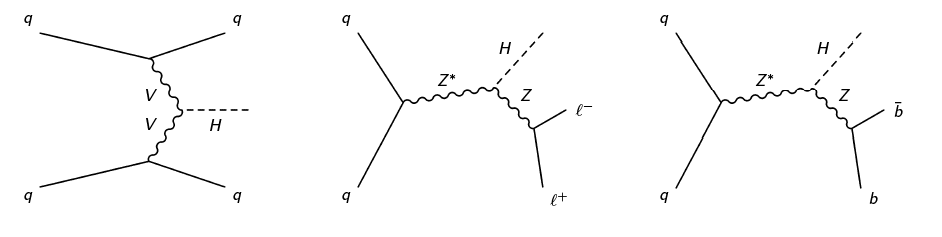
\includegraphics[width=\textwidth]{TalkPics/invcomb021213/feyndiags}
  %% \begin{fmfgraph*}(100,70)
  %%         \fmfleft{i1,i2}
  %%         \fmfright{o1,o2,o3}
  %%         \fmf{fermion}{i1,v1,o1}
  %%         \fmf{fermion}{i2,v2,o3}
  %%         \fmf{phantom,tension=4/5}{v1,v2}
  %%         \fmffreeze
  %%         \fmf{photon,label=$W,,Z$}{v1,v3}
  %%         \fmf{photon,label=$W,,Z$}{v2,v3}
  %%         \fmf{dashes}{v3,o2}
  %%         \fmflabel{$q$}{i1}
  %%         \fmflabel{$q$}{i2}
  %%         \fmflabel{$q$}{o1}
  %%         \fmflabel{$q$}{o3}
  %%         \fmflabel{$H$}{o2}
  %%       \end{fmfgraph*}
}
\date{}
\begin{document}
\begin{fmffile}{higgsexoupdatefeyndiags}

%TITLE PAGE
\section{Title}
\begin{frame}
  \titlepage
  
\end{frame}

\begin{frame}
  \frametitle{Overview}
  \begin{block}{}
    \scriptsize
    \begin{itemize}
    \item ARC author twiki has complete answers to most questions
    \item There are a couple of outstanding items: 
    \item[-] Lepton scale factor update and new PAS draft still ``to do''
    \item[-] We would like clarification for a few questions
    \item We also request your approval to make two analysis changes
    \item[-] Z extrapolation error: was under investigation previously
    \item[-] Top background method: change does not affect final limit
    \end{itemize}
  \end{block}
\end{frame}

\begin{frame}
  \frametitle{Items answered since we sent the twiki}
  \begin{block}{}
      \scriptsize
    \begin{itemize}
    \item Table of trigger fit parameters has been added
    \item[-] See backup
    \item EWK and QCD contributions to Z control region have been plotted separately
    \end{itemize}
  \end{block}
  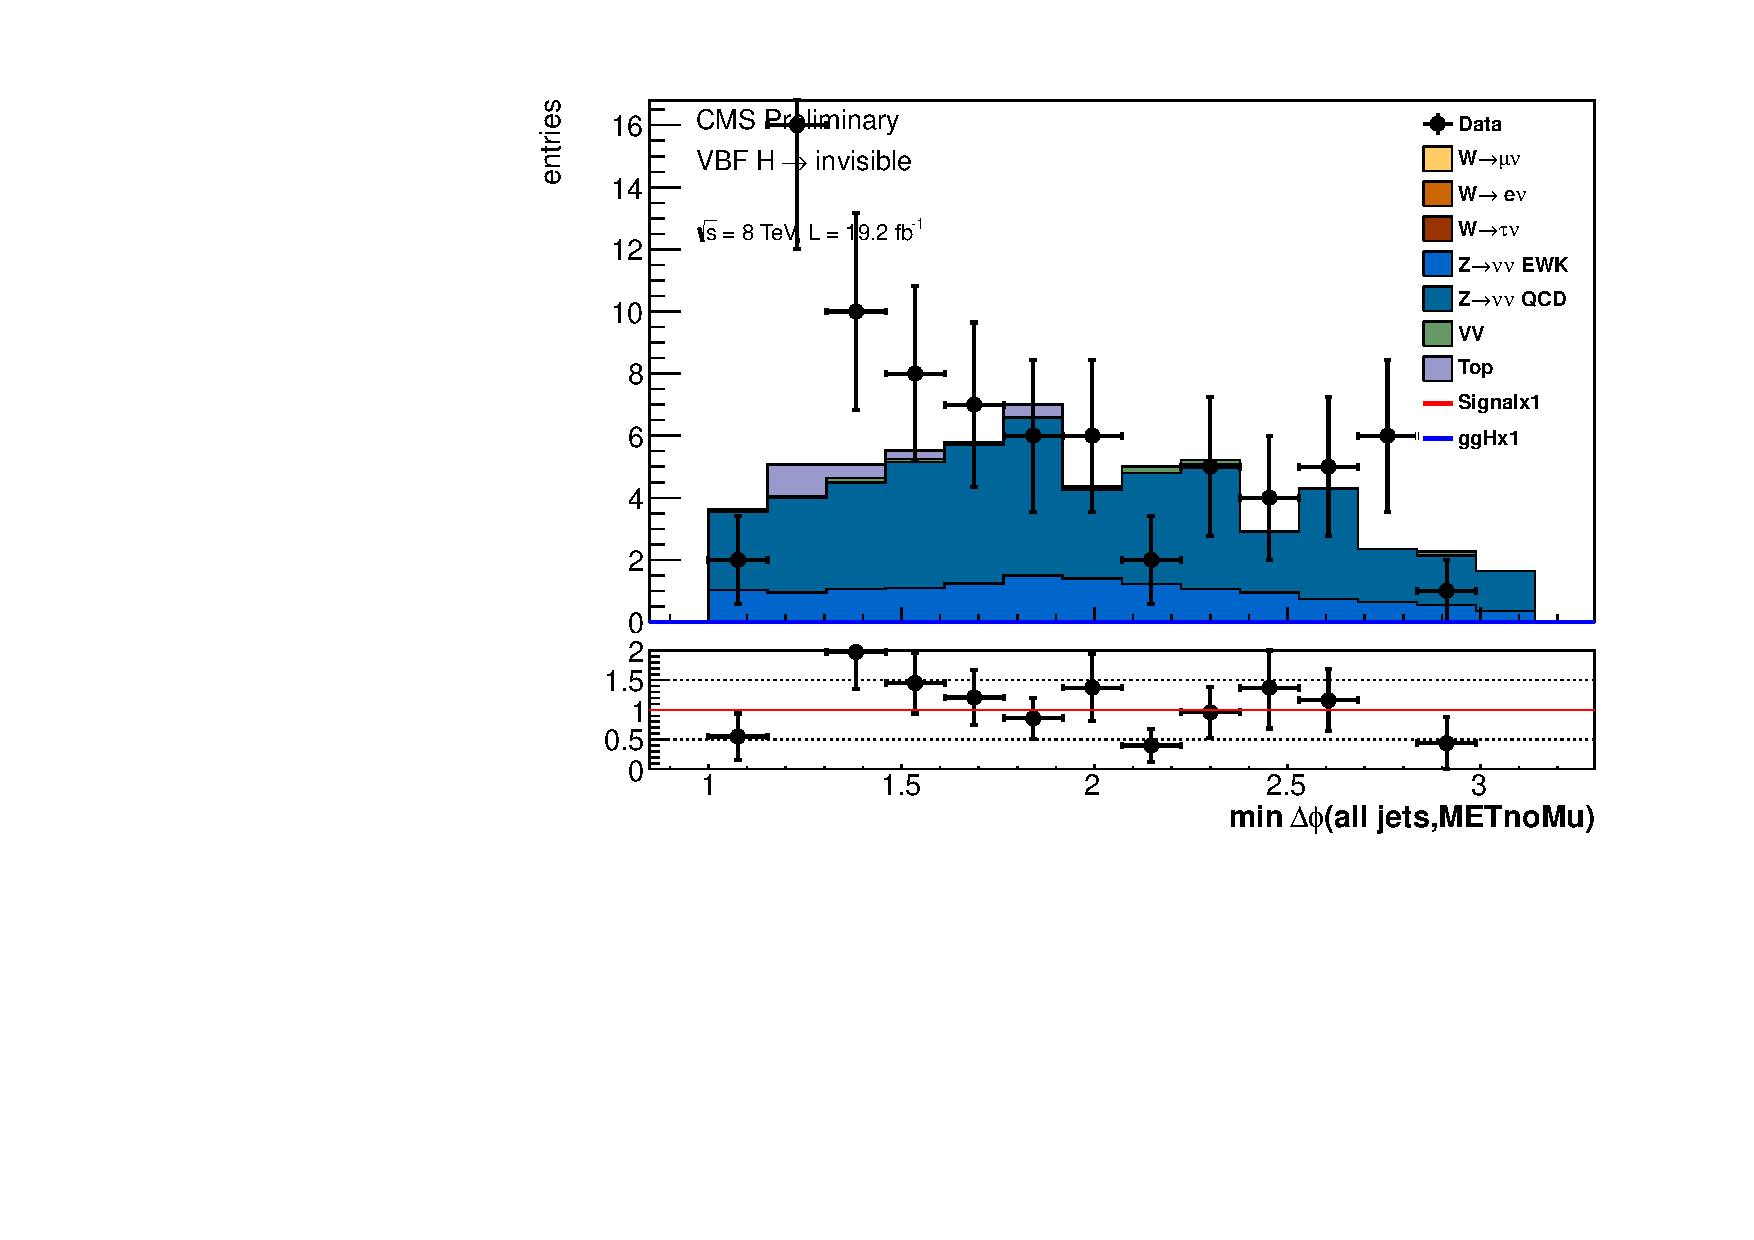
\includegraphics[clip=true,trim=0 0 0 20,width=.5\textwidth]{TalkPics/arcmeeting160215/mumu_alljetsmetnomu_mindphi.pdf}
  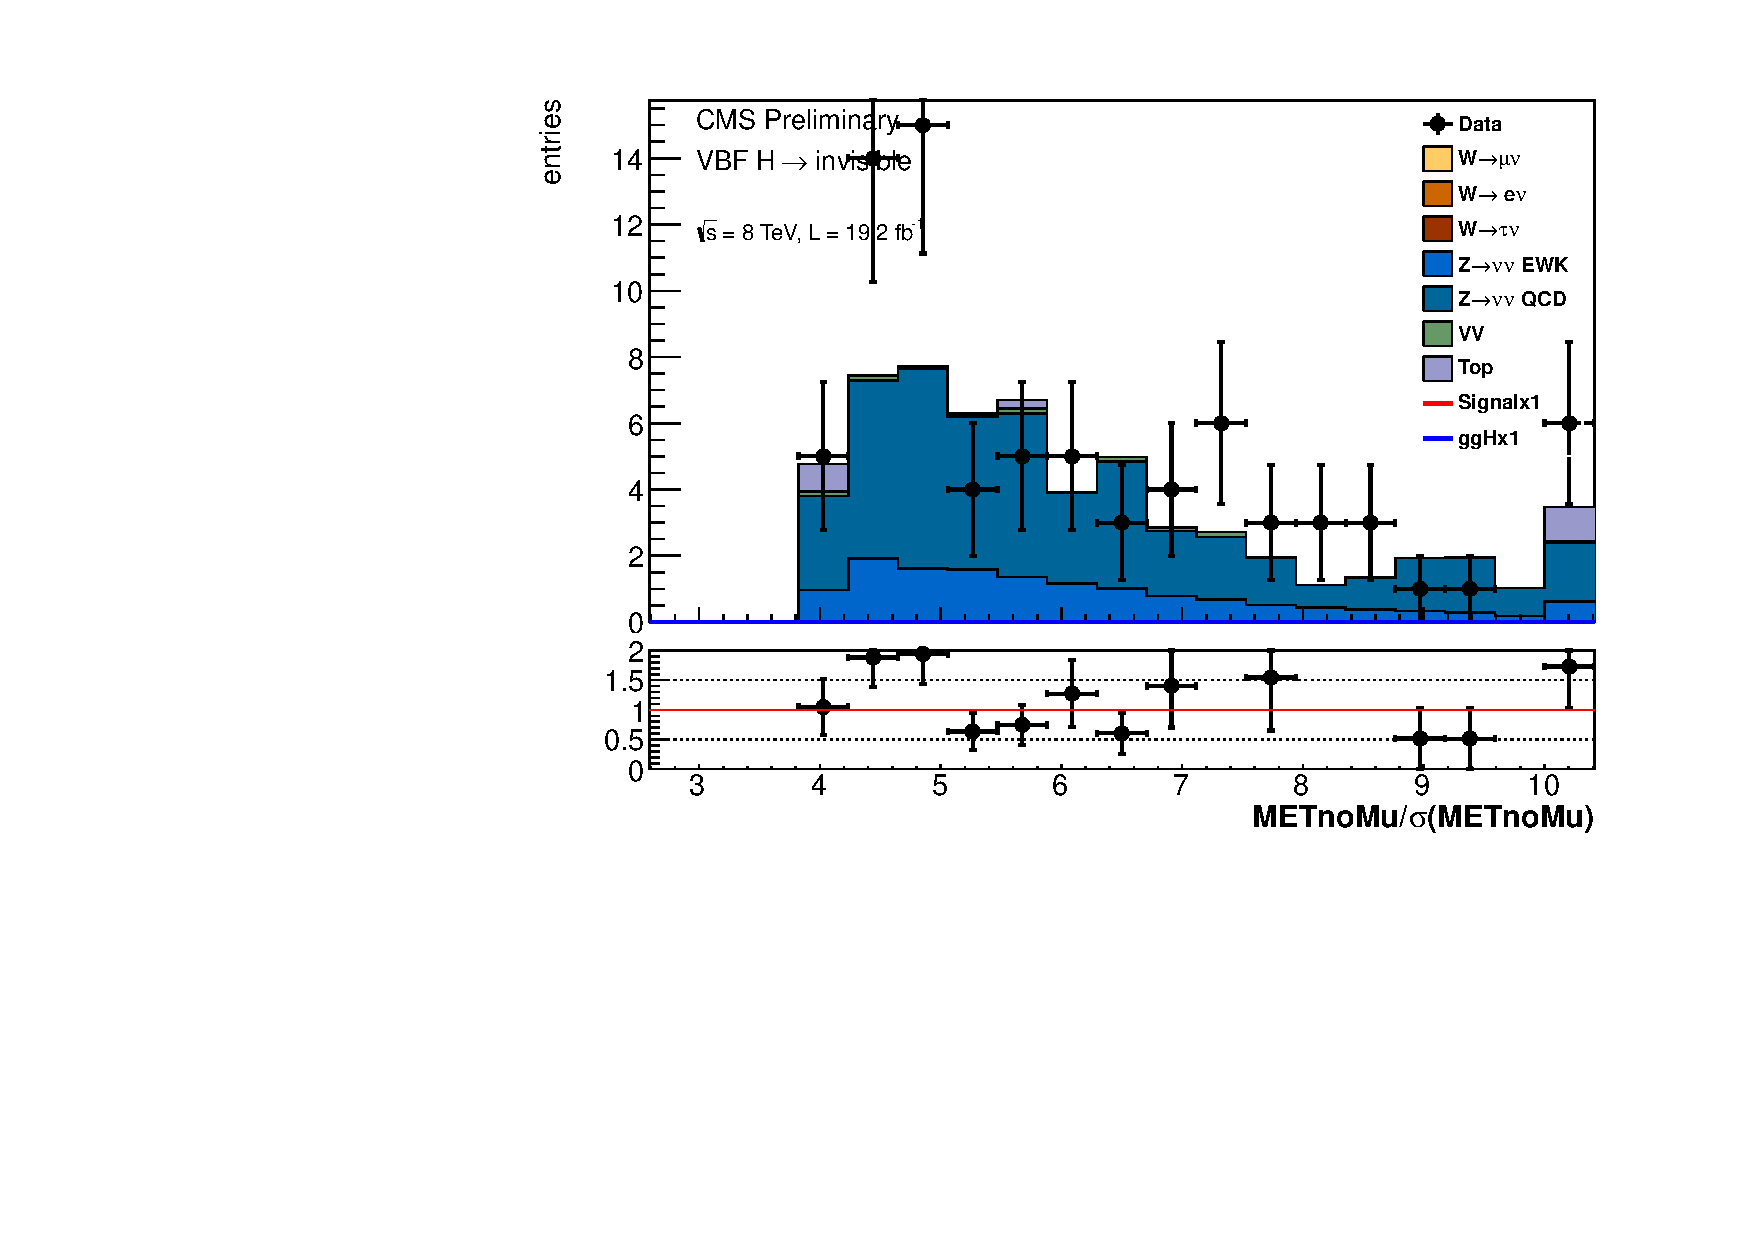
\includegraphics[clip=true,trim=0 0 0 20,width=.5\textwidth]{TalkPics/arcmeeting160215/mumu_metnomu_significance.pdf}
\end{frame}

\begin{frame}
  \frametitle{Items answered since we sent the twiki}
  \begin{block}{}
      \scriptsize
    \begin{itemize}
    \item A separated version of the likelihood scan plot has been produced
    \end{itemize}
  \end{block}
  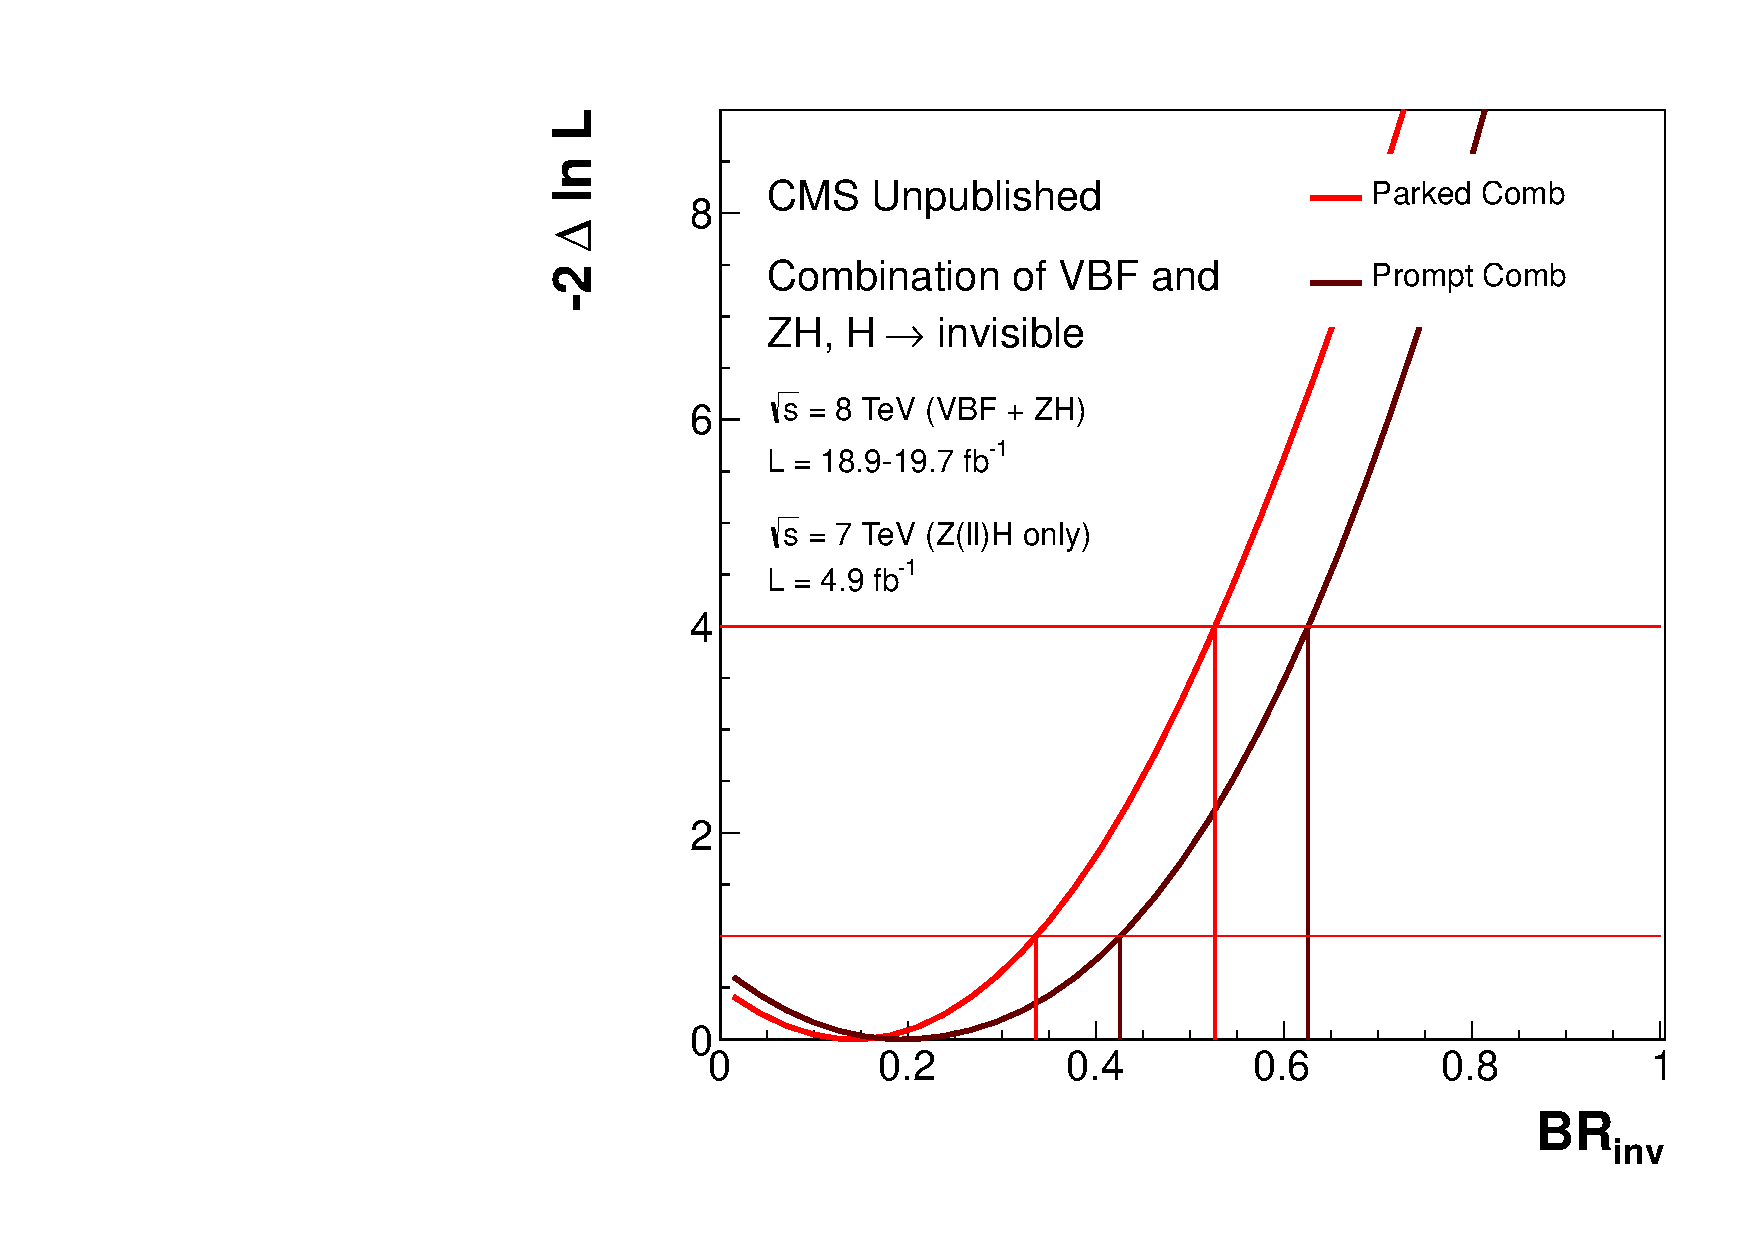
\includegraphics[clip=true,trim=0 0 0 20,width=.5\textwidth]{TalkPics/arcmeeting160215/combonlyscan.pdf}
  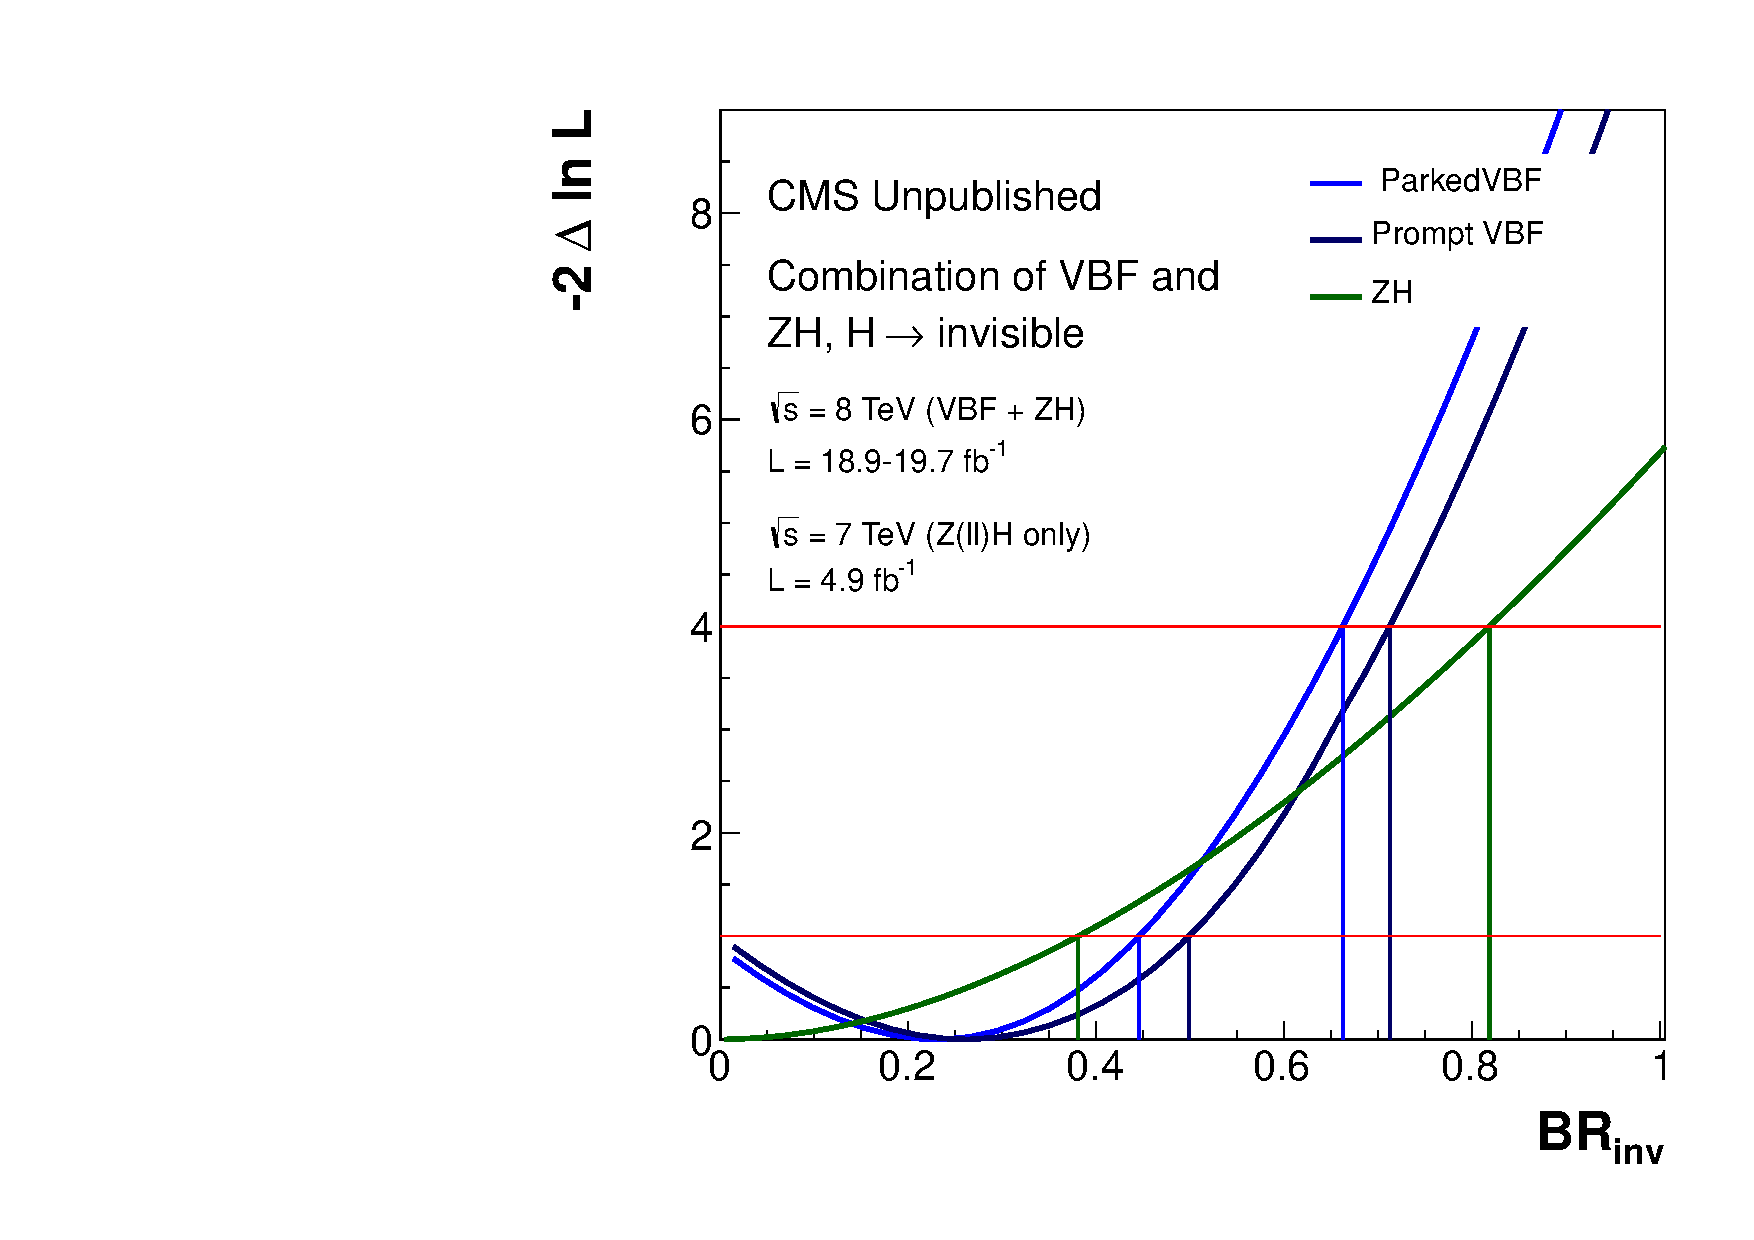
\includegraphics[clip=true,trim=0 0 0 20,width=.5\textwidth]{TalkPics/arcmeeting160215/individscan.pdf}
\end{frame}

\begin{frame}
  \frametitle{QCD in final plots}
  \begin{block}{}
    \scriptsize
    \begin{itemize}
    \item Three options:
    \item[1)] Just plot MC QCD ``out of the box''
    \item[-] Gives 20 events, close to 17 predicted
    \item[-] Didn't seem to have good agreement earlier in selection so hard to trust
    \end{itemize}
  \end{block}
  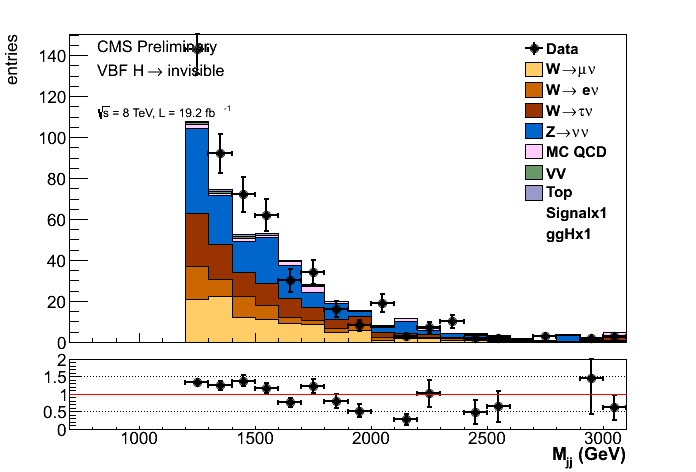
\includegraphics[clip=true,trim=0 0 0 20,width=.5\textwidth]{TalkPics/arcmeeting160215/nunu_withmcqcdraw_dijet_M.png}
  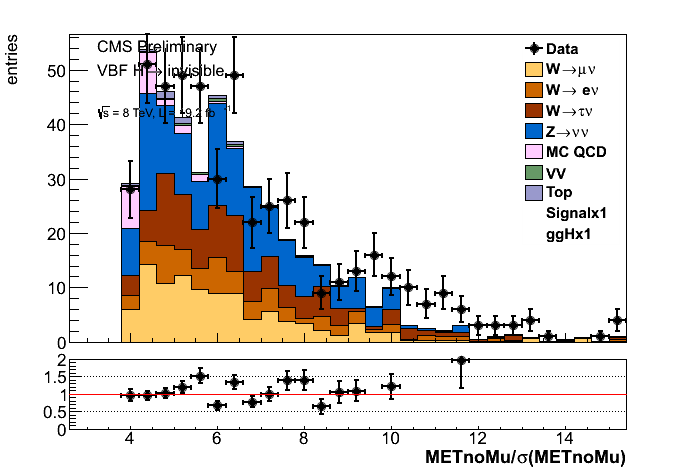
\includegraphics[clip=true,trim=0 0 0 20,width=.5\textwidth]{TalkPics/arcmeeting160215/nunu_withmcqcdraw_metnomu_significance.png}
\end{frame}

\begin{frame}
  \frametitle{QCD in final plots}
  \begin{block}{}
    \scriptsize
    \begin{itemize}
    \item[2)] MC QCD with inverted allmindphi $<$ 1.0 and mindphi(MET,j1/j2)$>$2.3, scaled to the expected 17 events (factor 0.04 scaling)
    \item[-] Still easy to produce
    \item[-] Looks very similar to full data driven method
    \end{itemize}
  \end{block}
  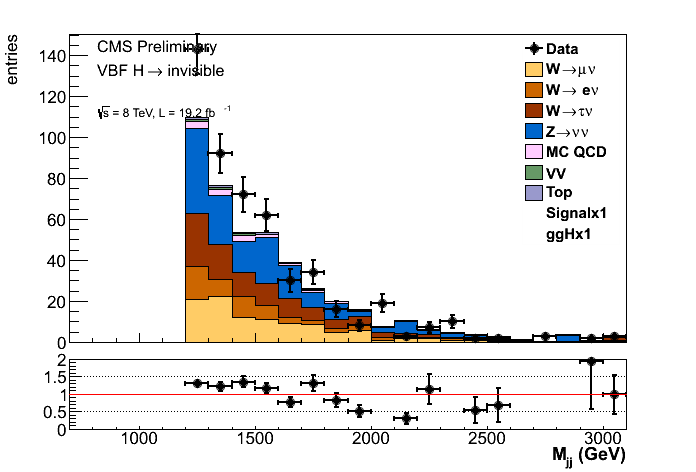
\includegraphics[clip=true,trim=0 0 0 20,width=.5\textwidth]{TalkPics/arcmeeting160215/nunu_withmcqcd_dijet_M.png}
  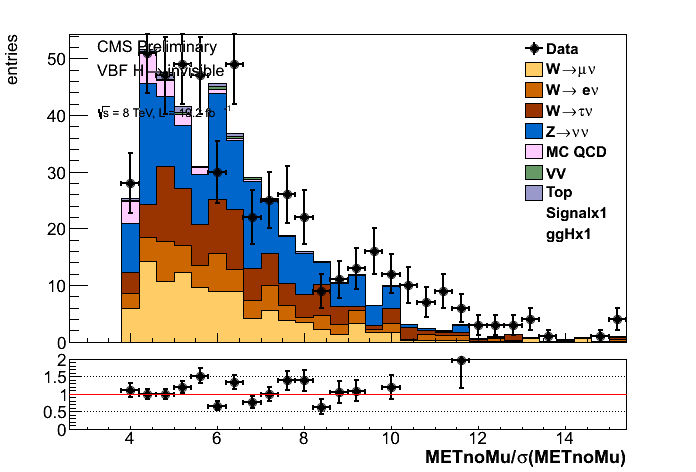
\includegraphics[clip=true,trim=0 0 0 20,width=.5\textwidth]{TalkPics/arcmeeting160215/nunu_withmcqcd_metnomu_significance.png}
\end{frame}

\begin{frame}
  \frametitle{QCD in final plots}
  \begin{block}{}
    \scriptsize
    \begin{itemize}
    \item[3)] Data driven estimate of QCD background shape
    \item[-] (inverted allmindphi $<$ 1.0 and mindphi(MET,j1/j2)$>$2.3), background subtracted and scaled with final scale factor (0.05)
    \end{itemize}
  \end{block}
  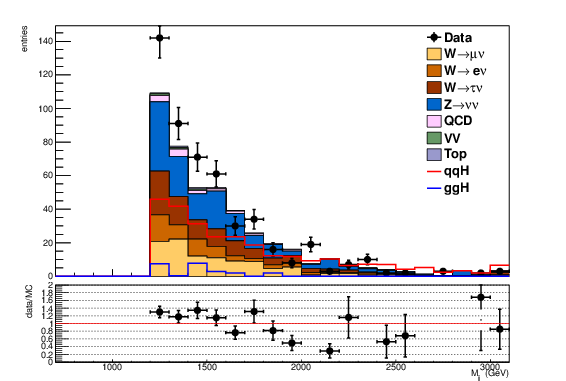
\includegraphics[clip=true,trim=0 0 0 20,width=.5\textwidth]{TalkPics/arcmeeting160215/nunu_withqcd_dijet_M.png}
  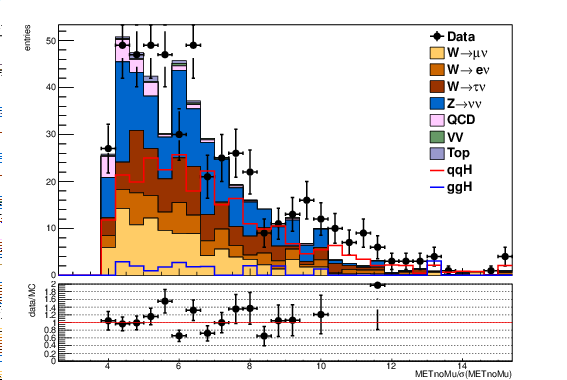
\includegraphics[clip=true,trim=0 0 0 20,width=.5\textwidth]{TalkPics/arcmeeting160215/nunu_withqcd_metnomu_significance.png}
\end{frame}



\begin{frame}
  \frametitle{Top background}
  \vspace{-.3cm}
  \begin{block}{}
    \scriptsize
    \begin{itemize}
    \item We discovered that the ttbar vs single top make up of the top contribution to our control and signal regions was quite different
      \vspace{-.1cm}
    \item[-] Signal region: 90\% single top, $W\rightarrow\tau\nu$ region: 30\% single top, top control region: $\sim$100\% ttbar
      \vspace{-.1cm}
    \item We therefore decided to investigate Wbb analysis based single top region
      \vspace{-.1cm}
    \item[-] Signal region + 1 tight e or $\mu$ + 1 of the VBF jets having a CSVM b-tag
      \vspace{-.1cm}
    \item[-] This region has 17\% single top
      \vspace{-.1cm}
    \item[-] Scale factor is compatible with 1: 0.88+-0.07(data stat.)+-0.08(MC stat.)
    \end{itemize}
  \end{block}
  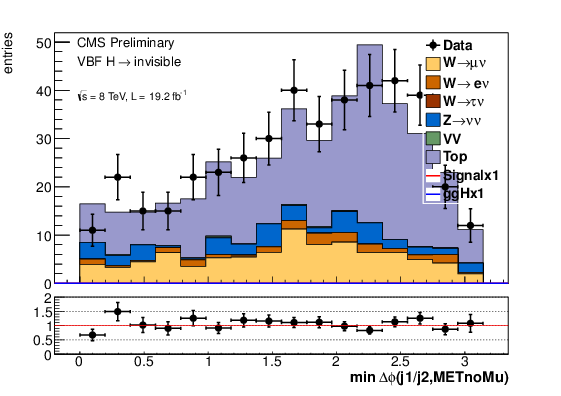
\includegraphics[clip=true,trim=0 0 0 20,width=.5\textwidth]{TalkPics/arcmeeting160215/top_jetmetnomu_mindphi.png}
  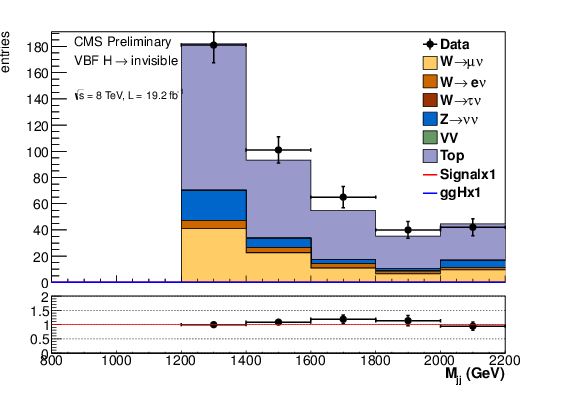
\includegraphics[clip=true,trim=0 0 0 20,width=.5\textwidth]{TalkPics/arcmeeting160215/top_dijet_M.png}
%!!PLOTS
\end{frame}

\begin{frame}
  \frametitle{Top background}
  \vspace{-.3cm}
  \begin{block}{}
    \scriptsize
    \begin{itemize}
    \item We also investigated adding ee+mumu to our control region
      \vspace{-.1cm}
    \item Added a Z mass window veto to avoid Z contamination
      \vspace{-.1cm}
    \item Gives 22 extra events (shown below left) which does not reduce the top uncertainty much as signal region MC statistics dominate
      \vspace{-.1cm}
    \item[-] 39\% down to 35\% not taking into account a systematic from Z mass window
      \vspace{-.1cm}
    \item Weight compatible with 1: 1.21+-0.19(data stat.)+-0.16(MC stat.)
      \vspace{-.1cm}
    \item For reference weight from emu region was also compatible with 1: 0.84+-0.19(stat.)+-0.14(MC stat.)
    \end{itemize}
  \end{block}
%!!PLOTS
  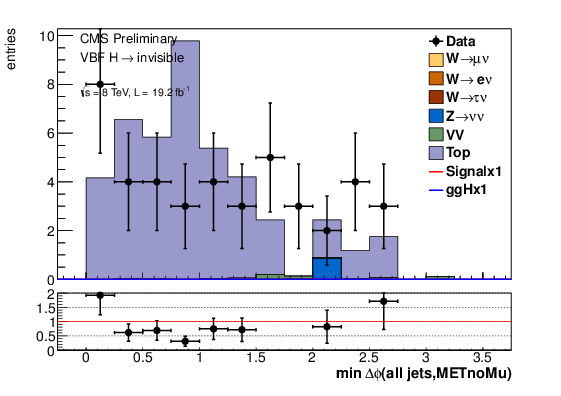
\includegraphics[clip=true,trim=0 0 0 20,width=.5\textwidth]{TalkPics/arcmeeting160215/topeemumuemu_alljetsmetnomu_mindphi.png}
  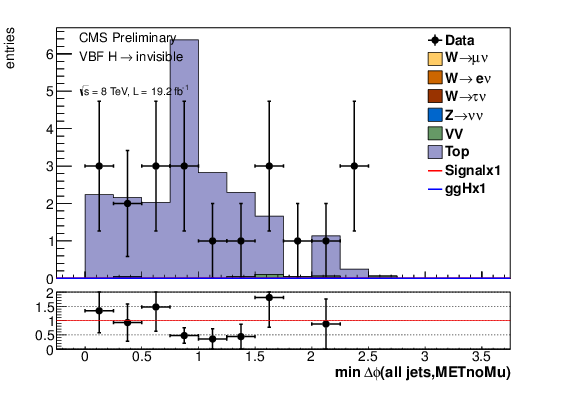
\includegraphics[clip=true,trim=0 0 0 20,width=.5\textwidth]{TalkPics/arcmeeting160215/top_alljetsmetnomu_mindphi.png}
\end{frame}

\begin{frame}
  \frametitle{$Z/\gamma^{*}\rightarrow\mu\mu$ to $Z\rightarrow\nu\nu$ extrapolation uncertainty}
  \begin{block}{}
    \scriptsize
    \begin{itemize}
    \item This was under study at the time of preapproval
    \item New studies with aMC@NLO\_MG5 show no evidence of incompatibility with result from MadGraph: 4\%
    \item Propose switching to stat uncertainty from MadGraph prediction
    \item[-] Already accounted for by MC stat uncertainty
    \item Details here: \url{https://indico.cern.ch/event/365513/contribution/0/material/slides/1.pdf}
    \end{itemize}
  \end{block}
\end{frame}

\begin{frame}
  \frametitle{Questions we have}
  \begin{block}{}
    \scriptsize
    \begin{itemize}
    \item Could you point us to a recipe for madgraph ttbar reweighting
    \item Could you advise us how to check EWK+QCD interference in Z background method
    \end{itemize}
  \end{block}
\end{frame}

\begin{frame}
  \frametitle{Summary}
  \label{lastframe}
  \begin{block}{}
    \scriptsize
    \begin{itemize}
    \item Almost all questions answered
    \item We request approval of our plans for the top background and Z uncertainty
    \item A couple of outstanding issues:
    \item[-] Lepton scale factors are being updated
    \item[-] PAS is being redrafted
    \end{itemize}
  \end{block}
\end{frame}

\begin{frame}
  \frametitle{Backup}
\end{frame}

\begin{frame}
  \tiny
  \begin{tabular}{|l|c|c|c|}
    \hline
    Region and run & Centre $x_0$ & Width $\Gamma$ & Maximum eff. $\varepsilon_{max}$ \\
    (units: GeV) & (GeV) & (GeV) & \\
    \hline
A: j2pt 40-50 , mjj 800-900 & $133 \pm 13$ & $1465 \pm 1101$ & $0.58 \pm 0.15$ \\
BC: j2pt 40-50 , mjj 800-900 & $101 \pm 5$ & $2351 \pm 1018$ & $0.61 \pm 0.04$ \\
D: j2pt 40-50 , mjj 800-900 & $133 \pm 22$ & $14972 \pm 9451$ & $0.82 \pm 0.12$ \\
    \hline
A: j2pt 40-50 , mjj 900-1000 & $112 \pm 42$ & $38 \pm 94580$ & $0.38 \pm 0.20$ \\
BC: j2pt 40-50 , mjj 900-1000 & $99 \pm 6$ & $1869 \pm 1317$ & $0.65 \pm 0.06$ \\
D: j2pt 40-50 , mjj 900-1000 & $106 \pm 6$ & $1910 \pm 1007$ & $0.76 \pm 0.05$ \\
    \hline
A: j2pt 40-50 , mjj 1000-5000 & $115 \pm 11$ & $40 \pm 508$ & $0.58 \pm 0.11$ \\
BC: j2pt 40-50 , mjj 1000-5000 & $119 \pm 5$ & $5503 \pm 1502$ & $0.84 \pm 0.04$ \\
D: j2pt 40-50 , mjj 1000-5000 & $112 \pm 6$ & $6636 \pm 2249$ & $0.91 \pm 0.05$ \\
    \hline
A: j2pt 50-60 , mjj 800-900 & $88 \pm 1$ & $1 \pm 78109$ & $0.30 \pm 0.02$ \\
BC: j2pt 50-60 , mjj 800-900 & $106 \pm 9$ & $9141 \pm 4207$ & $0.79 \pm 0.07$ \\
D: j2pt 50-60 , mjj 800-900 & $108 \pm 8$ & $5267 \pm 2795$ & $0.74 \pm 0.07$ \\
    \hline
A: j2pt 50-60 , mjj 900-1000 & $111 \pm 12$ & $1583 \pm 1518$ & $0.73 \pm 0.13$ \\
BC: j2pt 50-60 , mjj 900-1000 & $112 \pm 6$ & $19021 \pm 6743$ & $1.00 \pm 0.99$ \\
D: j2pt 50-60 , mjj 900-1000 & $109 \pm 9$ & $21363 \pm 9257$ & $1.00 \pm 0.76$ \\
    \hline
A: j2pt 50-60 , mjj 1000-5000 & $117 \pm 18$ & $3154 \pm 3282$ & $0.87 \pm 0.17$ \\
BC: j2pt 50-60 , mjj 1000-5000 & $111 \pm 4$ & $7182 \pm 1801$ & $0.95 \pm 0.03$ \\
D: j2pt 50-60 , mjj 1000-5000 & $111 \pm 4$ & $5918 \pm 1810$ & $0.97 \pm 0.03$ \\
\hline
A: j2pt 60-1000 , mjj 800-900 & $178 \pm 158$ & $100000 \pm 51037$ & $0.54 \pm 0.32$ \\
BC: j2pt 60-1000 , mjj 800-900 & $89 \pm 2$ & $3437 \pm 885$ & $0.79 \pm 0.02$ \\
D: j2pt 60-1000 , mjj 800-900 & $91 \pm 5$ & $7785 \pm 2715$ & $0.79 \pm 0.04$ \\
    \hline
A: j2pt 60-1000 , mjj 900-1000 & $92 \pm 5$ & $865 \pm 835$ & $0.64 \pm 0.07$ \\
BC: j2pt 60-1000 , mjj 900-1000 & $86 \pm 2$ & $6737 \pm 1440$ & $0.97 \pm 0.02$ \\
D: j2pt 60-1000 , mjj 900-1000 & $86 \pm 2$ & $2881 \pm 803$ & $0.90 \pm 0.02$ \\
    \hline
A: j2pt 60-1000 , mjj 1000-5000 & $89 \pm 3$ & $3025 \pm 1091$ & $0.96 \pm 0.03$ \\
BC: j2pt 60-1000 , mjj 1000-5000 & $51 \pm 4$ & $11294 \pm 1888$ & $0.97 \pm 0.01$ \\
D: j2pt 60-1000 , mjj 1000-5000 & $61 \pm 3$ & $12774 \pm 1882$ & $0.99 \pm 0.01$ \\
\hline
\end{tabular}
\end{frame}

\end{fmffile}
\end{document}
